\chapter{Environment per Sistemi Esperti}
Il numero di ambienti di sviluppo per sistemi esperti è cresciuto negli anni e con esso il numero e la tipologia di funzionalità offerte. Le prime \emph{shell} erano semplici metodi di rappresentazione della conoscenza basata sull'uso delle regole, con il supporto di strumenti di inferenza piuttosto limitati. Con gli anni, la lista e la tipologia di funzionalità offerte si è arricchita introducendo una varietà di possibilità per la rappresentazione della conoscenza, strategie di ricerca, meccanismi specializzati di inferenza e strumenti di supporto allo sviluppo dei sistemi.

L'evoluzione di questi sistemi è stata motivata con il tempo e la quantità di sforzo richiesto per la costruzione di sistemi esperti usando linguaggi tradizionali e sistemi strettamente vincolati all'uso della regole per la rappresentazione della conoscenza.

L'obiettivo inseguito con l'evoluzione degli ambienti di sviluppo era quello di ridurre i tempi ed i costi di sviluppo dei sistemi esperti. Inoltre l'uso di questi strumenti ha garantito:
\begin{itemize}
	\item un miglioramento generale della qualità e l'affidabilità dei sistemi prodotti
	\item di astrarre l'attività di sviluppo del sistema esperto da quelle relative allo sviluppo dell'ambiente di base
	\item agli ingegneri della conoscenza la possibilità di focalizzarsi sugli aspetti correlati alla modellazione degli elementi del dominio del sistema esperto
	\item di utilizzare strumenti rapidi per l'acquisizione e la modifica della conoscenza dei sistemi esperti
\end{itemize}

I miglioramenti hanno incrementato in questo modo le possibilità di successo nello sviluppo di sistemi esperti. Come ulteriore effetto, il ridursi della complessità generale delle operazioni realizzazione ha consentito di gestire e produrre soluzioni di sempre maggiore complessità.

\section{Evoluzione degli strumenti di sviluppo}
Tornando indietro agli albori della produzione di sistemi esperti, i meccanismi di inferenza e le basi di conoscenza erano strettamente accoppiati fra loro. La prima generazione di sistemi non era altro che grandi applicazioni scritte in linguaggi come LISP. Nonostante tutti i linguaggi di programmazione possano essere utilizzati per la produzione di sistemi esperti, alcuni di essi offrivano caratteristiche che rendevano la stessa attività più agevole. Esempi di linguaggi largamente utilizzati per queste attività sono il linguaggio LISP e Prolog. Purtroppo, la quantità di tempo e sforzo richiesto per la produzione usando queste tipologie di linguaggi diventava rapidamente insostenibile con l'aumentare della complessità. Inoltre, l'accoppiamento fra funzionalità necessarie all'inferenza e quelle per la rappresentazione e la gestione della conoscenza non permetteva una distinzione di ruoli fra gli ingegneri di sistema e quelli della conoscenza.

\subsection{Expert System Shell}

Questo approccio alla lavorazione venne superato nella successiva generazione. Durante la creazione di sistemi esperti di seconda generazione come MYCIN, i ricercatori si accorsero dell'importanza di implementare i sistemi in modo che fosse possibile una separazione, più o meno netta, fra la base di conoscenza e i meccanismi per la sua rappresentazione dalle funzionalità atte all'implementazione del motore inferenziale e i meccanismi dello stesso.

Rimuovendo la conoscenza di dominio da questi sistemi vennero realizzati i primi sistemi di tipo \emph{Skeletal Shell} o \emph{Expert System Shell} utilizzando gli strumenti sviluppati nel progetto originale e inserendo nuova conoscenza di dominio era possibile creare una grande verità di nuovi sistemi esperti con un sforzo relativamente ridotto. I sistemi di seconda generazione di maggior successo hanno dato vita a \emph{Shell} per lo sviluppo di sistemi esperti. Sono esempi EMYCIN, KAS e EXPERT: rispettivamente questi ultimi vennero prodotti rimuovendo le conoscenze di dominio da MYCIN, PROSPECTOR e CASNET.

Sebbene l'utilizzo di questi strumenti velocizzasse la produzione di nuovi sistemi di diversi ordini di magnitudine, la necessità di attenersi alle strategie utilizzate nei sistemi originali rappresentava un limite alla flessibilità del sistema. Spesso le \emph{Shell} fornivano strumenti integrati e strutture che rendevano lo sviluppo dei sistemi molto più semplice ed immediato, ma limitavano le classi di problemi a cui potevano essere applicati e riducevano grandemente le scelte di design possibili per il realizzatore di sistemi esperti. \cite{development1993}

\subsection{Expert System Environment}

Il successivo passo negli strumenti di sviluppo per sistemi esperti è quello costituito dalla produzione delle prima serie di \emph{Environment per Sistemi Esperti}. L'idea alla base di questa generazione di tool era quella di realizzare delle \emph{Shell} che offrissero sistemi multipli per la rappresentazione della conoscenza, l'inferenza e il controllo insieme ad un completo ambiente di sviluppo \cite{development1993}, senza però limitare le scelte di design dei realizzatori.

Questi strumenti vennero ulteriormente arricchiti con l'integrazione di funzionalità orientate allo sviluppo come meccanismi di tracciamento delle regole e strutture per il debugging dei sistemi. Esempi di \emph{Environment} creati sono OPS5, OPS83, CLIPS, JESS.

L'utilizzo di questi sistemi si poneva come punto d'incontro fra le due generazioni precedenti: come mostrato in \figurename~\ref{fig:classificazione-tools}, nonostante l'utilizzo degli \emph{Environment} facilitasse lo sviluppo dei sistemi esperti, non riduceva la flessibilità e le opzioni di design a disposizione dello sviluppatore come per gli strumenti di seconda generazione. Spesso lo sviluppo di questi sistemi richiedeva ancora un certo grado di esperienza nell'uso di linguaggi di programmazione e conoscenze sintattiche in quanto gli ambienti ereditavano sintassi e strutture già a disposizione nei linguaggi di prima generazione (la famiglia di environment OPS ereditava una sintassi simile a quella usata in LISP \cite{brownston1985}).

\begin{figure}
\centering
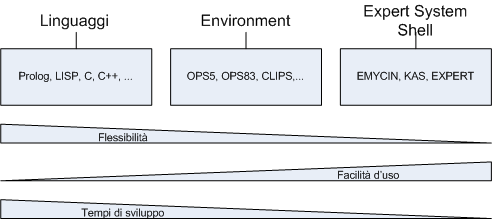
\includegraphics[scale=0.7]{Immagini/Capitolo1/classificazione-strumenti.png}
\caption{Classificazione dei tool di sviluppo per sistemi esperti}\label{fig:classificazione-tools}
\end{figure}

\section{Rappresentazione della conoscenza}
Con il termine \emph{Rappresentazione della conoscenza} ci si riferisce alle modalità con le quali la conoscenza è strutturata ed organizzata in un sistema. Fra le modalità di rappresentazione più note supportate dai tool di sviluppo per sistemi esperti sono annoverabili \emph{Regole}, \emph{Reti semantiche}, \emph{Frame} e \emph{Oggetti}. Ognuna di queste tecniche presenta vantaggi e svantaggi: alcune permettono una estrema facilità di modifica e comprensione dei sistemi, mentre altre consentono un'alta efficienza d'uso della memoria. Un ideale environment per sistemi esperti dovrebbe provvedere a supportare il maggior numero possibile di queste tecniche di rappresentazione della conoscenza \cite{development1993}, per offrire una più ampia possibilità di scelta agli sviluppatori durante le fasi di design dei sistemi.

\subsection{Regole}
La più nota forma di rappresentazione della conoscenza è quella basata su regole. \'E probabilmente un assioma dell'intelligenza artificiale, e della moderna psicologia, che comportamenti ritenuti intelligenti siano governati da regole. Anche nel mondo, le persone tendono ad associare intelligenza con coerenza nei comportamenti, e spesso il concetto di comportamento viene spiegato facendo riferimento a quello di regolarità. \cite{jackson1999}

Le \emph{regole di produzione} sono un formalismo utilizzato, in origine, nello studio delle macchine astratte, delle grammatiche formali e nella progettazione dei linguaggi di programmazione. Successivamente il loro utilizzo è approdato nell'ambito dei sistemi esperti e dell'intelligenza artificiale. Nella letteratura tecnica sono anche identificate come \emph{Regole condizione-azione} o \emph{Regole situazione-azione}. Questa nomenclatura risulta appropriata in quanto le regole sono spesso utilizzate per rappresentare, in forma codificata, associazioni fra \emph{Pattern}\footnote{Con il termine \emph{Pattern} si fa riferimento schemi di caratteristiche richieste ad un insieme di elementi} di dati presenti nel sistema e sequenze di azioni che il sistema stesso dovrebbe eseguire come conseguenza di un riscontro. Conseguentemente la funzione delle regole è precisamente quella di specificare regole di comportamento: forniti insiemi di dati (astraendo dalla particolare interpretazione), determinano i risultati da concretizzare.

Le produzioni sono realmente regole per la manipolazione di stringhe di simboli, chiamate spesso regole di riscrittura. Post ha studiato le proprietà dei sistemi a regole basati su produzioni, che lui stesso ha chiamato \emph{Sistemi Canonici}. Questi ultimi sono definiti come un tipo di sistemi formali basato su:

\begin{itemize}
	\item un \emph{alfabeto} A per la creazione di stringhe
	\item un insieme di stringhe considerati come \emph{assiomi}
	\item un insieme di produzioni nella forma: 
	\[
	\alpha_1\$_1 \cdots \alpha_m\$_m \rightarrow \beta_1\$_1^{'} \cdots \beta_n\$_n^{'}
	\]	
	dove
	\begin{itemize}
		\item ogni elemento $\alpha_i$ e $\beta_1$ rappresenta una stringa
		\item gli elementi $\alpha_1$ e $\alpha_m$ sono spesso nulli
		\item alcuni o addirittura tutti gli elementi $\alpha_i$ o $\beta_1$ possono essere nulli
		\item ogni $\$_i$ rappresenta una stringa variabile (che può essere la stringa nulla)
		\item ogni elemento $\$_i$ è sostituito da uno $\$_i^{'}$.
	\end{itemize}
\end{itemize}

Nell'ambito specifico dei sistemi esperti, le regole normalmente determinano come le strutture simboliche che rappresentano lo stato corrente del sistema debbano essere manipolate per avvicinare la rappresentazione stessa dello stato ad una soluzione. L'attivazione progressiva delle regole produce una \emph{catena di inferenza}.

Il concetto di regole utilizzato  all'interno dei sistemi esperti differisce da quello generico di produzioni come regole di riscrittura sotto aspetti superficiali, ma mantengono gli stessi principi fondamentali e le stesse proprietà formali.

Se da una parte nelle produzioni come regole di riscrittura l'interesse è focalizzato sulla grammatica della struttura dei simboli \emph{per se}, nell'uso delle regole come mezzi di rappresentazione della conoscenza nei sistemi esperti l'interesse è concentrato sul processo di trasformazione di una istanza del problema originale in un forma che ne rappresenti una soluzione.

Conseguentemente l'alfabeto dei \emph{sistemi canonici} è rimpiazzato da un vocabolario di simboli o atomi e da una grammatica relativamente semplice per la generazione di strutture simboliche. Normalmente il vocabolario consiste di tre insiemi:

\begin{itemize}
	\item un insieme $N$ di nomi di oggetti del dominio
	\item un insieme $P$ di nomi di proprietà che specificano attributi di un oggetto
	\item un insieme $V$ di valori che questi attributi possono assumere.
\end{itemize}

Generalmente la grammatica utilizzata prevede la specifica di triple \emph{oggetto-attributo-valore}, ma questo assunto non lede la possibilità di specifiche più espressive.

Una volta descritto un vocabolario di simboli e una grammatica per la generazione di strutture simboliche, è possibile generare una codifica della descrizione di uno stato iniziale di un problema di interesse. Questa descrizione, costituita da strutture simboliche, corrisponderà esattamente agli assiomi previsti nella definizione di \emph{sistema canonico}. La descrizione originale del problema verrà progressivamente riscritta tramite una serie di applicazioni.

Un sistema a produzioni consiste di un \emph{rules-set} (spesso anche definito come \emph{memoria delle produzioni}), un \emph{rules-interpreter} che verifica l'applicabilità delle regole e una memoria di lavoro. Il ruolo di quest'ultima componente è quella di memorizzare la descrizione iniziale del sistema, così come la descrizione finale attesa e gli stati intermedi prodotti durante la fase di elaborazione. La possibilità di attivazione delle regole è governata dall'interprete, il quale confronta la descrizione intermedia del sistema con l'insieme di regole e decide quale applicare. L'applicazione stessa delle regole (in un processo analogo a quello descritto per la riscrittura simbolica) modifica ulteriormente la descrizione del sistema presente nella \emph{working memory}.

Schematicamente questo processo può essere descritto nella forma generale
\[
C_1, \cdots, C_n \rightarrow A_1, \cdots, A_n
\]
interpretabile come:
\begin{quote}
	{\bfseries [if]} le condizioni $C_1$ e $\cdots$ e $C_n$ sono vere,\\
	{\bfseries [then]} esegui le azioni $A_1$ e $\cdots$ e $A_n$.
\end{quote}

Con i termini \emph{left-hand side} e \emph{right-hand side} si è soliti indicare rispettivamente la porzione di condizione e quella di azione di una regola.

\subsection{Reti semantiche}
Un'altra tecnica di rappresentazione della conoscenza usa reti di strutture chiamate appunto \emph{reti semantiche}. I nodi di queste reti sono costituiti da eventi, oggetti o concetti, che possono essere relazionati fra loro, tramite l'uso di archi di varia natura, per stabilire strutture gerarchie fra i concetti stessi. \cite{development1993}

Due relazioni molto comuni in questo tipo di rappresentazione sono quelle di tipo \emph{is-a} e \emph{has-part}. L'utilizzo di questa forma di rappresentazione permette una memorizzazione efficiente delle proprietà dei concetti in quanto, data la natura gerarchica implicitamente indotta dalle relazioni di ereditarietà, i nodi posti al più basso livello della rete eviteranno la ridefinizione di proprietà già deducibili dai concetti ai quali questi ultimi sono relazionati.

La definizione offerta da \emph{R. H. Richens}, ideatore delle \emph{reti semantiche}, spiega le stesse come
\begin{quote}
''una \emph{interlingua} nella quale tutte le peculiarità strutturali del linguaggio di base sono rimosse e siamo lasciati con solo quello che io chiamo una \emph{rete semantica} di \emph{idee spoglie}. In questa rete gli elementi rappresentano cose, qualità o relazioni $\cdots$[ o] punti di collegamento fra cose verso le proprie qualità o relazioni, o da qualità e relazioni verso un'ulteriore qualificazione''\cite{richens1956}
\end{quote}

\subsection{Frame}
Il concetto di ereditarietà introdotto tramite l'utilizzo delle \emph{reti semantiche} viene ulteriormente esteso tramite l'utilizzo del concetto di \emph{Frame}. 
\begin{quote}
''Un \emph{frame} è una struttura dati per la rappresentazione di situazioni stereotipate. [\dots] Diverse tipologie di informazioni vengono collegate a ciascun frame. Alcune di queste informazioni riguardano l'utilizzo dello stesso. Altre sono a proposito di quello che ci si può attendere. Altre riguardano cosa fare se queste attese non sono confermate. \cite{minsky1974}''
\end{quote}

La struttura dei \emph{frame} può essere immaginata come una rete di nodi e relazioni. I nodi principali, posti alla testa della gerarchia, sono fissi e rappresentano concetti ed informazioni che sono assiomaticamente veri in una situazione. A questi nodi vengono collegati, nei livelli via via più bassi, diversi \emph{terminali}. Questi ultimi rappresentano \emph{slot} che devono essere riempiti da specifiche istanze o dati. Ogni terminale ha la possibilità di specificare condizioni che devono risultare verificare per permettere la modifica o l'accesso ai dati contenuti negli slot. 

Le forme più semplici di condizioni possono richiedere l'intervento dell'utente per fornire dati da assegnare a specifici slot, condizioni più complesse possono invece essere utilizzate per collegare fra loro informazioni disponibili in diversi altri terminali. 

Il contenuto degli slot può essere un informazione atomica, così come un'ulteriore sotto struttura \emph{frame}. L'utilizzo di strutture innestate permette la creazione di ulteriori livelli gerarchici con estrema facilità. \cite{minsky1974} 

\subsection{Oggetti}
Gli oggetti nell'approccio \emph{object-oriented} alla rappresentazione della conoscenza descrivono una strategia di rappresentazione derivata da quella dei \emph{frame}. Dal quest'ultima eredita i concetti di relazione, slot e l'organizzazione gerarchica fra gli elementi stessi \cite{holsapple1994object}.

L'innovazione introdotta dall'approccio basato su oggetti è quella consentire la comunicazione fra gli oggetti stessi attraverso un protocollo basato sullo scambio di messaggi: in seguito alla ricezione di un messaggio, un oggetto attiva una appropriata procedura e valuta se propagare o meno il messaggio ad altri oggetti con cui lo stesso è in relazione \cite{development1993}. 

Il paradigma basato su oggetti realizza una modalità generale di rappresentazione della conoscenza e per la sua manipolazione. La sua importanza è data sia dalla capacità di caratterizzazione della conoscenza, sia dalla varietà di tecniche che questo tipo di formalismo consente di integrare all'interno di ogni genere di sistema \cite{holsapple1994object}.

\section{Meccanismi di inferenza}
La componente principale di un qualsiasi strumento di sviluppo per sistemi esperti, sia esso un linguaggi classico di programmazione, sia esso una \emph{shell} o un \emph{environment}, risiede nel motore inferenziale.

Esso può essere descritto come il cuore di ogni sistema esperto: è il componente con il compito di contenere e gestire la conoscenza necessaria al raggiungimento della soluzione del problema che il sistema esperto punta a risolvere, oltre che gestire l'ordine con il quale applicare la conoscenza di dominio al servizio del raggiungimento di un obiettivo.

Il componente genericamente identificato come \emph{motore inferenziale} è in realtà una sintesi del lavoro svolto da due componenti separate interne allo stesso: l'\emph{interprete} e lo \emph{scheduler}\cite{development1993}.

\paragraph{Interprete} Il ruolo dell'interprete può essere descritto nei termini del ciclo \emph{recognize-act}. Lo stesso è un processo iterato suddiviso in tre fasi consecutive ed eseguito con l'obiettivo di manipolare la descrizione del problema contenuta nella memoria di lavoro. Le fasi che costituiscono il ciclo \emph{recognize-act} possono essere riassunte nelle seguenti:
\begin{list}{}{}
	\item[(1)] \emph{Confrontare} gli elementi della memoria di lavoro (la descrizione parziale dello stato del problema) con l'elenco dei \emph{Pattern} presenti nella porzione \emph{LHS} di ogni regola disponibile nel \emph{rules-set}.
	\item[(2)] Valutare l'elenco delle regole le cui condizioni risultano completamente soddisfatte e selezionarne una\footnote{La restrizione di selezione di una singola regola fra quelle applicabili può anche essere sostituita da strategie di gestione dei conflitti che prevedono la selezione di un gruppo di regole fra le applicabili, come mostrato da \cite{Doorenbos95productionmatching}} da applicare.
	\item[(3)] Applicare la regola: l'applicazione consiste nell'esecuzione di ognuna delle azioni contenute nella porzione \emph{RHS} della regola
\end{list}

La fase (2) dell'interprete è delegata alle funzioni dello \emph{Scheduler}. 

\paragraph{Scheduler} Le funzioni svolte dallo \emph{Scheduler} sono quelle di decidere l'ordine di applicazione di porzioni di conoscenza di dominio \cite{development1993}. Facendo riferimento ad un ipotetico motore inferenziale che utilizza una strategia di controllo basata su regole, questo componente utilizza una serie di criteri eseguendo una selezione fra le attivazioni disponibili. Le euristiche utilizzate per la selezione possono essere incluse in origine nell'ambiente di sviluppo o richiedere l'intervento dello sviluppatore per essere specificate.

\'E questo l'elemento a creare la differenza fra logiche di controllo \emph{globali} e \emph{locali}. 

\subparagraph{Logiche globali} Le prime rappresentano un gruppo di strategie indipendenti dal dominio applicativo, normalmente incluse negli ambienti di sviluppo, e che non richiedono l'intervento dello sviluppatore. L'unica possibilità offerta è quella di scegliere una fra diverse strategie, ammesso che più di una venga fornita dal sistema. La personalizzazione della sequenza di esecuzione viene quindi delegata ad apposite strategie di controllo basate su rappresentazioni specifiche dei dati nella \emph{working memory}. Un esempio di \emph{environment} ad utilizzare questo genere di strategie globali è CLIPS.

Spesso, le strategie di controllo della catena di inferenza sono il sunto della combinazione di differenti meccanismi di base, ognuno dei quali si basa su differenti proprietà. Le buone prestazioni di un sistema esperto spesso dipendono da proprietà chiave di questi regimi di controllo \cite{jackson1999}, come la \emph{sensibilità} o la \emph{stabilità}.
\begin{quote}
	''Un sistema a produzioni il quale dimostri reattività alle necessità del suo ambiente si può affermare che dimostri \emph{sensibilità}. Uno che è capace di mantenere una continuità nei suoi comportamenti, può essere detto che mostri \emph{stablità}.''\cite{McDermott:1977:PSC:1045343.1045364}
\end{quote} 
La prima indica la capacità di una logica di adattarsi con rapidità a modifiche dell'ambiente che si riflettono nelle descrizioni nella memoria di lavoro, la seconda indica il grado di coerenza nella linea di ragionamento.\cite{jackson1999}

Nonostante i meccanismi di risoluzione dei conflitti variano molto da sistema a sistema, la popolarità di alcune caratteristiche presenti in molti di essi richiede un approfondimento:

\begin{itemize}
	\item \emph{Refrattarietà}: proprietà che non consente ad una attivazione di essere eseguita più di una volta sullo stesso gruppo di dati. Se più attivazioni con gli medesimi dati vengono riscontrate, sono semplicemente ignorate.
	\item \emph{Attualità}: agli elementi all'interno della memoria di lavoro vengono applicati delle etichette temporali. Le attivazioni vengono successivamente selezionate utilizzando i tag applicati.
	\item \emph{Specificità}: le attivazioni vengono selezionate in base a criteri legati alla specificità dei pattern che trovano riscontro con la descrizione presente nella memoria di lavoro
\end{itemize}

\subparagraph{Logiche locali} Le strategie di controllo \emph{locali} offrono un più alto grado di personalizzazione allo sviluppatore, ma con esso anche maggiori responsabilità. \'E infatti responsabilità dei designer quella di specificare un apposito insieme di \emph{meta-regole} che consentano la discriminazione delle attivazioni in cerca della più opportuna da attivare per ogni stato del sistema. La selezione viene eseguita basandosi sulla conoscenza di dominio inserita all'interno delle \emph{meta-regole}. Un esempio di sistema ad utilizzare questa tipologia di \emph{Scheduler} è MYCIN.

\subsection{Controllo basato su regole}
Storicamente, i primi ambienti per lo sviluppo ad essere implementati si basavano sulla specifica degli elementi di conoscenza attraverso la codifica in formato di regole di produzione.

Le strategie di ricerca sviluppate per il controllo dell'inferenza in questa categoria di sistemi si basano spesso su metodi come il \emph{Forward Chaining} e il \emph{Backward Chaining}.

\paragraph{Forward chaining}
Il \emph{forward chaining} può essere descritto come applicazione ripetuta del \emph{modus ponens}\footnote{Nella logica, il Modus ponens è una regola di inferenza riassumibile con: \begin{quote}
Se \emph{p implica q} è una proposizione vera e anche la premessa \emph{p} è vera, allora la conseguenza \emph{q} è vera.
\end{quote}}. Partendo da una serie di condizioni la cui validità è assiomatica o appurata, il sistema crea una catena di inferenza estraendo nuova conoscenza da quella disponibile fino a quando una descrizione della soluzione non viene individuata, un obiettivo non è stato raggiunto o non è possibile effettuare ulteriore inferenza.

Nei motori inferenziali che utilizzano questa strategia di controllo, il \emph{rules-set} viene scansionato alla ricerca di regole la cui parte \emph{condizione} (o \emph{LHS}) non risulti verificata dalla descrizione dello stato disponibile nella memoria di lavoro. Una volta identificato almeno un riscontro, è possibile logicamente concludere che la parte conseguente (la porzione \emph{RHS}) risulterà anch'essa verificata nella descrizione dello stato. L'applicazione della parte \emph{azione} produrrà una modifica della descrizione dello stato\footnote{La modifica dello stato avviene solitamente attraverso l'asserzione o la ritrattazione di fatti nella \emph{working memory}.}.

La concatenazione in avanti è un esempio del concetto generale di \emph{ragionamento guidato dai dati}, un tipo di ragionamento in cui l'attenzione parte dai fatti conosciuti. Ogni volta che nuova informazioni viene aggiunta, una certa quantità di ragionamento viene generato e guidato dai dati aggiunti. Il maggior pericolo derivante da questo tipo di inferenza è che un enorme numero di conseguenze irrilevanti possa distogliere l'attenzione da un numero ridotto di conseguenze invece rilevanti e indispensabili per giungere ad una soluzione del problema. \cite{russellnorvig2009}

\paragraph{Backward chaining}
L'algoritmo di concatenazione all'indietro, o \emph{Backward chaining}, parte da una conclusione desiderata (un obiettivo, una descrizione della soluzione di un problema) e lavora a ritroso scansionando tutta la base di conoscenza alla ricerca di implicazioni che verifichino la conclusione desiderata: qualora tutte le precondizioni dell'implicazione individuata risultino vere allora anche la conclusione risulterà vera, in caso contrario il processo di ricerca a ritroso verrà ripetuto per le precondizioni non soddisfatte.

La concatenazione all'indietro è una forma di ragionamento basato sugli obiettivi. Spesso il costo dell'utilizzo di questa strategia di inferenza è inferiore rispetto a quello tramite l'utilizzo della \emph{forward chaining} in quanto il processo coinvolge solo i fatti rilevanti. \cite{russellnorvig2009}

\subsection{RETE: matching fra regole e stato}
L'algoritmo di \emph{Forward chaining} rappresenta una modalità di inferenza progettata per risultare di facile comprensione ed utilizzo. Porta con se però tre criticità di grande rilevanza: \cite{russellnorvig2009}
\begin{itemize}
	\item il ciclo interno dell'algoritmo prevede la ricerca di tutti gli unificatori tali che una la premessa di una regola possa trovare riscontro con un insieme adeguato di dati presenti nella \emph{working memory}. Questa operazione è definitia \emph{Pattern Matching}.
	\item per ogni iterazione, la ricerca nel \emph{rules-set} deve essere ripetuta completamente anche nei casi in cui le modifiche alla \emph{working memory} sono di piccola entità.
	\item l'impostazione stessa dell'algoritmo comporta il rischio di generazione di un grande numero di dati irrilevanti per il raggiungimento dell'obiettivo.
\end{itemize}

Prendendo in esame una ipotetica configurazione di una regola in cui la precondizione sia costituita da un singolo \emph{pattern}, la verifica dell'applicabilità della regola prevede la ricerca all'interno della \emph{working memory} di un singolo elemento in grado di verificare la condizione. L'operazione, se eseguita in un base di conoscenza opportunamente indicizzata, può essere completata in tempo costante per ogni fatto. \cite{russellnorvig2009}

Aumentando il numero di pattern presenti all'interno della porzione \emph{LHS} di una regola, il confronto va eseguito per ogni pattern individualmente. In seguito, qualora sia necessario eseguire dei test di coerenza per verificare il binding delle variabili comuni a più pattern, l'operazione di confronto va ripetuta per ogni possibile combinazione dei fatti individuati dalle singole condizioni.

L'algoritmo RETE si propone come una soluzione efficiente per il problema di pattern matching. Proposto per la prima volta nel 1979 dal C. L. Forgy \cite{forgy1979} \cite{forgy1982}, l'algoritmo affronta il problema partendo da una semplice considerazione: l'applicazione di una regola genera piccoli cambiamenti nello stato del sistema e spesso questi cambiamenti minimi non richiedono una valutazione completa dell'intero \emph{rules-set}. Le criticità principali di una formulazione na\"{\i}ve di un algoritmo di matching derivano proprio dalla necessità di eseguire una scansione completa dell'intera base di conoscenza e dell'intera memoria di lavoro per ogni cambiamento dello stato del sistema.

La soluzione propone i miglioramenti sintetizzandoli in due cambiamenti principali:
\begin{itemize}
	\item evitare di scansionare l'intera \emph{working memory} per trovare nuovi riscontri per i singoli pattern
	\item evitare di scansionare l'intero \emph{rules-set} per trovare nuove attivazioni
\end{itemize}

La scansione dell'intera \emph{working memory} viene evitata memorizzando in una unità di memoria dedicata per ogni pattern la lista di elementi che risultano coerenti con il pattern stesso. Queste unità di memoria vengono aggiornate in linea con i cambiamenti della \emph{working memory}.

Quando un nuovo elemento viene asserito e quindi entra a far parte della descrizione dello stato fornita dalla \emph{working memory}, l'algoritmo esegue una valutazione di ogni pattern singolarmente per il nuovo elemento aggiunto ed, solo in caso di verifica positiva, l'elemento stesso viene inserito all'interno dell'unità di memoria locale \cite{forgy1982}.

Quando un elemento fuoriesce dalla \emph{working memory}, lo stesso viene rimosso da tutte le unità di memoria locali dei pattern in cui l'elemento è memorizzato. Il processo di ricerca può avvenire ripetendo nuovamente le verifiche per i singoli pattern \cite{forgy1982} oppure, più efficientemente, tenendo in una porzione di memoria separata una lista di riferimenti fra elementi e le memorie in cui essi sono contenuti \cite{Doorenbos95productionmatching}.

La scansione dell'intero \emph{rules-set} viene evitata attraverso l'utilizzo di una struttura a grafo per la rappresentazione delle regole. In seguito ad una fase di compilazione, la porzione \emph{LHS} delle regole viene scomposta nei singoli pattern. Per ognuno di essi viene realizzata, qualora non fosse possibile condividere una struttura analoga creata precedentemente, un circuito di nodi in grado di eseguire dei test su singoli elementi della \emph{working memory}. Come ultimo elemento del circuito viene aggiunta una unità di memoria locale, denominata \emph{Alpha-Memory}, la quale accoglierà l'insieme di elementi che, singolarmente, hanno verificato l'elenco di condizioni che il circuito descrive \cite{Doorenbos95productionmatching}.

L'insieme di circuiti derivanti dalla compilazione dei singoli pattern prende il nome di \emph{Alpha-Network}.

Una seconda porzione della rete è quella nota con il nome di \emph{Beta-Network}. In questa sezione vengono eseguiti i test di coerenza sul binding delle variabili fra le condizioni. Durante la fase di compilazione, una volta create le porzioni \emph{alpha} di ogni singolo pattern, quelli appartenenti alla stessa \emph{LSH} vengono collegati fra loro attraverso l'uso di speciali nodi, chiamati \emph{Join-Node}. Questi nodi, oltre a riunire singoli pattern in una catena che rappresenti l'intera \emph{LHS}, hanno il compito di eseguire l'insieme di test necessari alle verifiche di coerenza sul binding delle variabili, dove necessario. Qualora i test eseguiti in questi nodi a due input risultino positivi, viene creata una struttura che contiene i due elementi della memoria di lavoro che sono risultati coerenti e la stessa memorizzata all'interno di una unità di memoria agganciata direttamente al \emph{Join-Node}. 

\begin{figure}
\centering
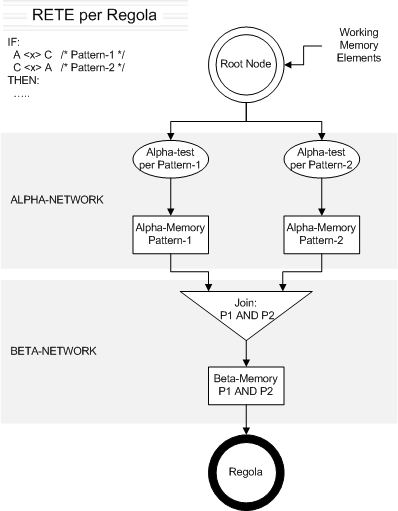
\includegraphics[scale=0.7]{Immagini/Capitolo1/grafico-regola-rete.png}
\caption{Grafico ottenuto dalla compilazione di una regola}\label{fig:grafico-regola}
\end{figure}


La struttura prende il nome di \emph{Token}\footnote{Nella formulazione dell'algoritmo proposto originariamente in \cite{forgy1979} e \cite{forgy1982} con il termine \emph{Token} si faceva riferimento a una descrizione di un cambiamento nella \emph{working memory}, notificato ai nodi componenti la rete tramite l'uso di \emph{tag}. La formulazione proposta in \cite{Doorenbos95productionmatching} utilizza l'appellativo per indicare una sequenza di \emph{working memory elements} che abbiano verificato una porzione della \emph{beta-network}. Il concetto di tag, usati nella prima formulazione per indicare il tipo di modifica che il \emph{token} rappresentava, nella seconda formulazione è completamente assente}.

L'utilizzo di un ulteriore tipo di memoria nella \emph{Beta-Network}, chiamata appunto \emph{Beta-Memory}, consente di memorizzare attivazioni parziali che risultano valide solo per una porzione della regola in attesa che, tramite l'asserzione di ulteriori fatti, l'intera regola risulti attivabile.

Il processo di trasformazione delle regole porta a due benefici sostanziali:
\begin{itemize}
	\item la compilazione dei singoli pattern eseguita per la formazione dell'\emph{alpha-network} consente di partizionare la working-memory in frammenti di minore dimensioni. Questo si traduce in un minor numero di confronti durante i test di coerenza. Inoltre, pattern simili presenti in più regole vengono accorpati e rappresentati da un unico circuito \emph{alpha}. La fase di valutazione verrà eseguita soltanto una volta per tipo di pattern.
	\item gruppi di pattern simili, analogamento a quanto descritto nel punto precedente, vengono accorpati in un solo circuito \emph{beta}, riducendo ulteriormente i costi delle verifiche per i test di coerenza.
\end{itemize}

Il processo di creazione della rete può avvenire attraverso un reale processo di compilazione \cite{forgy1982} che prevede la conversione dell'intero \emph{rules-set} in una sequenza di istruzioni ed espressioni che rappresentino le varie condizioni (implementazione \emph{compilata}), oppure attraverso un processo di creazione di una rappresentazione esplicita di grafo nelle modalità citate poc'anzi (implementazione \emph{interpretata}). 

Il vantaggio della prima variante è la maggiore velocità, in contrasto al maggior consumo di memoria e alla difficoltà di implementazioni di procedure in grado di alterare la struttura della rete durante l'esecuzione attraverso l'aggiunta o la rimozione di produzioni \cite{Doorenbos95productionmatching}.

La seconda variante rende più semplice l'implementazione di procedure di manipolazione della rete e risulta di globalmente di più facile implementazione e comprensione. Purtroppo questi vantaggi prevedono un \emph{trade-off} di tipo prestazionale \cite{Doorenbos95productionmatching}.

\section{Lo scenario attuale}
Il numero soluzioni commerciali e libere per lo sviluppo di sistemi esperto è estremamente elevato. Nonostante questo, nell'ambito dello sviluppo accademico le soluzioni individuate con maggior frequenza si restringono a due sistemi: CLIPS e JESS \cite{laerhoven1999}.

\subsection{CLIPS}
CLIPS è l'acronimo di C Language Integrated Production System: un linguaggio di programmazione sviluppato al NASA Johnson Space Center nella metà del 1980. Prende spunto da tool come OPS5 e ART, supportandone le caratteristiche di maggior importanza e introducendone di nuove come le funzionalità relative alla programmazione procedurale, supportanto una sintassi simile a quella LISP. Lo sviluppo iniziò in un contesto in cui erano emergenti, ma ancora costose, soluzioni di environment basati su linguaggio C. Il risultato è il sistema meno costoso e di maggiore reperibilità al mondo, non meno efficiente di soluzioni commerciali alternative disponibili. La prima versione non integrava funzionalità chiave introdotte solo successivamente, come il linguaggio procedurale e il paradigma di programmazione ad oggetti \cite{jackson1999}.

\subsection{JESS}
Nato originariamente come un clone di CLIPS, JESS è un environment per sistemi esperti scritto in Java con l'obiettivo di estendere l'ambito di utilizzo dell'environment verso l'integrazione con tecnologie per il web basate su Java, come gli applet. Il numero di funzionalità originariamente offerte era un set limitato di quelle offerte da CLIPS, con il tempo lo sviluppo si è diretto verso l'aggiunta di funzionalità originali in maniera indipendente dal progetto padre, separando in questo modo i due progetti.

\subsection{Integrazione}
Le possibilità di integrazione fra environment per sistemi esperti e applicazioni tradizionali è un ambito non ancora completamente esplorato. Se prendiamo in considerazione ambiti orientati al Web, queste possibilità di ricerca si espandono ulteriormente.

Le possibilità offerte dall'utilizzo di un linguaggio tanto versatile quanto lo è Java, hanno mostrato nuovi scenari di integrazione non ancora esplorati fino a questo momento.

Solo prendendo in esame l'ambito dello sviluppo orientato ai servizi per il web, lo scenario attuale mostra un ridotto numero di sistemi disponibili rispetto a quelli tradizionali individuabili \cite{dokas2005}.

Purtroppo, l'architettura e il linguaggio di programmazione utilizzati da CLIPS rendono l'integrazione con applicazioni scritte in linguaggi di alto livello o orientate al web di difficile utilizzo. Sebbene JESS sia una alternativa più comoda in questo ambito, restrizioni di licenza ne limitano l'utilizzo.

\section{Obiettivi di questa tesi}
Questa tesi si prefigge l'obiettivo di progettare e quindi implementare un environment per sistemi esperti basato su linguaggio interpretato Python e che offra un set di funzionalità simili a quelle offerte da CLIPS.

Allo scopo di valutarne le possibilità di integrazione in scenari differenti, verrà inoltre progettata un'interfaccia di utilizzo dello stesso utilizzando il protocollo XMLRPC.

